\chapter{Universal approximation in 1D}
\label{sec:universal_approximation}

\begin{supportbox}{About this chapter}
While formally proving the universal approximation theorem is beyond the scope of this book, it is helpful to get an intuitive feeling for how such proofs can be constructed. In this appendix we follow and extend the visual intuitions from a 2019 online book chapter by M. Nielsen,\footnote{\url{http://neuralnetworksanddeeplearning.com/chap4.html}} to which we refer for an extended discussion (and some interactive visualizations), especially for the case of multi-dimensional inputs.
\end{supportbox}

We focus on the original approximation theorem by Cybenko \cite{cybenko1989approximation} which considers models having one hidden layer with sigmoid activation functions. We also restrict the analysis to functions with a single input and a single output, that can be visualized easily. The reasoning can be extended to other activation functions and to higher dimensions.

The outline of this visual proof is relatively simple: 

\begin{enumerate}
\item As a first step, we show how to manually set the weights of a model with a single neuron in the hidden layer to approximate a step function.
\item Then, we proceed to show how adding another unit in the hidden layer allows to approximate any function which is constant over a small interval, and zero everywhere else (we call these interval functions “bin” functions). 
\item Finally, we describe a simple procedure to approximate a generic function by first binning it to the desired accuracy, and then adding as many neurons as needed to approximate all bins in turn. For $m$ bins we obtain a network with $2m$ neurons. For a generic function with multiple inputs, this number would grow exponentially in the number of dimensions, making the proof non constructive in a practical case.
\end{enumerate}

\section{Approximating a step function}

To begin, let us consider a single neuron in the hidden layer, in which case we can write the network’s equation as (ignoring the output bias term, as it is not helpful in our derivation):
%
$$
f(x)=a\sigma(wx+s)
$$
%
For the purposes of visualization, we rewrite this by adding a minus sign on the bias, and we factor the multiplication term on the entire input of $\sigma$ (the two variants are clearly equivalent):
%
\begin{equation}
f(x) = \eqnmarkbox[drawred]{node}{a}\sigma(\eqnmarkbox[drawgreen]{node2}{w}(x-\eqnmarkbox[drawblue]{node3}{s}))
\label{eq:proof_1}
\end{equation}
\annotate[yshift=-1em]{below,left}{node}{Amplitude}
\annotate[yshift=-1em]{below,right}{node2}{Slope}
\annotate[yshift=-1em]{below,right}{node3}{Shift}

\vspace{1em}
This is similar to the “tunable” variant of sigmoid we introduce in Section \ref{sec:activation_functions}. In particular, in this formulation $\color{drawred}a$ controls the amplitude of the sigmoid, $\color{drawgreen}w$ controls the slope, and $\color{drawblue}s$ shifts the function by a fixed amount.

\begin{SCfigure}
    \centering
    \hspace{1em}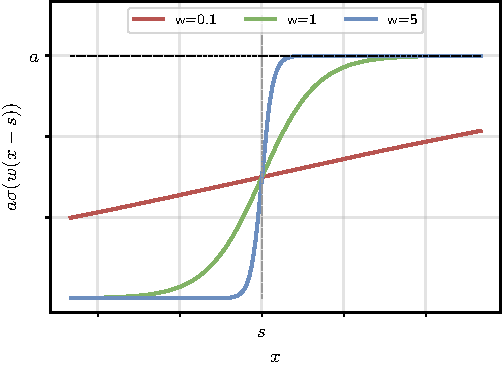
\includegraphics[width=0.5\textwidth]{images/tunable_sigmoid.pdf}
    \caption{A network with a single neuron in the hidden layer can be visualized as a sigmoid with controllable slope, center, and amplitude. We show here an example where we fix the amplitude and the center, but we vary the slope.}
    \label{fig:tunable_sigmoid}
\end{SCfigure}
%
We show in Figure \ref{fig:tunable_sigmoid} several plots of \eqref{eq:proof_1}, where we fix $a$ and $s$ while varying $w$. As can be seen, by increasing $w$ the slope gets steeper. Fixing it to a very large constant (say, $w=10^4$), we are left with a very good approximation to a step function, of which we can control the location of the step (the $s$ parameter) and the amplitude (the $a$ parameter), as shown in Figure \ref{fig:step_function}.

\begin{figure}
    \centering
    \begin{subfigure}[b]{0.32\textwidth}
    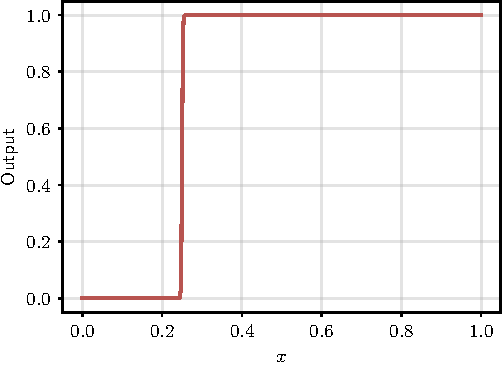
\includegraphics[width=0.95\textwidth]{images/step_function.pdf}
    \caption{1 neuron}
    \label{fig:step_function}
    \end{subfigure}
    \hfill
    \begin{subfigure}[b]{0.32\textwidth}
    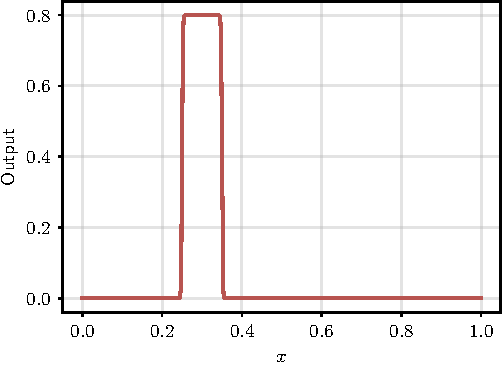
\includegraphics[width=0.95\textwidth]{images/bin.pdf}
    \caption{2 neurons}
    \label{fig:bin_function}
    \end{subfigure}
    \begin{subfigure}[b]{0.32\textwidth}
    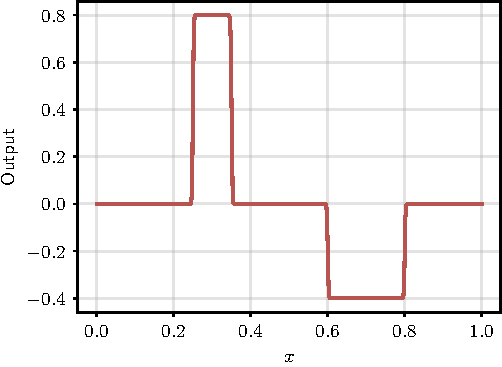
\includegraphics[width=0.95\textwidth]{images/bin_2.pdf}
    \caption{4 neurons}
    \label{fig:bin_function_2}
    \end{subfigure}
    \caption{(a) A neural network with one input, one hidden neuron, and one output can approximate any step function (here shown with $a=1$ and $s=0.3$). (b) With two hidden neurons and one output we can approximate any function which is constant over a small interval. (c) With four neurons, we can approximate any function which is piecewise constant over two non-zero intervals. Note that bins can be negative by defining a negative amplitude.}
\end{figure}

\section{Approximating a constant function}

If we add a second neuron with opposite amplitude (and slightly shifted position), we can approximate a function which is constant over a small interval (we call it a “bin” function). Defining a width $\Delta$ we can write:

\begin{equation}
f(x) = a\sigma\left(w\left(x-\eqnmarkbox[drawred]{node}{s -\frac{\Delta}{2}}\right)\right)  -a\sigma\left(w\left(x-\eqnmarkbox[drawgreen]{node2}{s+\frac{\Delta}{2}}\right)\right)
\label{eq:proof_2}
\end{equation}
\annotate[yshift=-1em]{below,left}{node}{Go up [down] at $s-\frac{\Delta}{2}$}
\annotate[yshift=-1em]{below,right}{node2}{Go down [up] at $s+\frac{\Delta}{2}$}

\vspace{1em}
where we recall that $w$ is now a large constant, e.g., $10^4$. \eqref{eq:proof_2} describes a function (equivalent to a model with one hidden layer having two neurons) which increases by $a$ at $s-\frac{\Delta}{2}$, is constant with value $f(x)=a$ over the interval $\left[s-\frac{\Delta}{2}, s+\frac{\Delta}{2}\right]$, and then decreases to $0$ afterwards. An example is  shown in Figure \ref{fig:bin_function}.

For the following, we can rewrite the previous function as $f(x; a, s, \Delta)$ to highlight the dependence on the three parameters $a$, $s$, and $\Delta$.

\section{Approximating a piecewise constant function}

Because $f_{a, s, \Delta}(x)$ is effectively $0$ outside the corresponding interval, two functions defined over non-intersecting intervals will not influence each other, i.e., the “bin” function we just defined is highly localized. Hence, by adding two additional neurons in the hidden layer we can define a function which is constant over two separate intervals (an example of which is shown in Figure \ref{fig:bin_function_2}):
%
$$
f(x)=f(x;a_1,s_2,\Delta_1)+f(x;a_2,s_2,\Delta_2)
$$
%
The rest of the proof is now trivial and proceeds by binning the function we want to approximate in many small intervals. Given any (continuous) function $g(x)$ over an interval (which we assume $[0,1]$ for simplicity), we first bin the input domain into $m$ equispaced intervals, where $m$ controls the accuracy of the approximation (the higher $m$, the better the approximation). Hence, the $i$-th bin spans the interval:
%
$$
B_i = \left[\frac{i}{m}-\frac{\Delta}{2}, \frac{i}{m}+\frac{\Delta}{2}\right]
$$
%
where $\Delta$ is the size of each bin. For each bin, we compute the average value of $g(x)$ inside the interval itself:
%
$$
g_i = \frac{1}{\Delta}\int_{x \in B_i} g(x)dx
$$
%
Finally, we define a network with $2m$ neurons in the hidden layer, two for each bin. Each bin function is centered in the bin and takes value $g_i$:
%
\begin{equation}
f(x)=\sum_{i=1}^m f\left(x; \eqnmarkbox[drawgreen]{node2}{g_i}, \eqnmarkbox[drawred]{node}{\frac{i}{m}},\Delta\right)
\label{eq:proof_3}
\end{equation}
\annotate[yshift=-1em]{below,right}{node}{The $i$-th bin is centered in $\frac{i}{m}$}
\annotate[yshift=-1em]{below,left}{node2}{(Approximated) constant value}

\newpage
We show in Figure \ref{fig:sin_approximation} an example of such approximation in the case of $g(x)=\frac{\sin(x)}{x}$ for increasing number of bins ($m=5$, $m=15$, $m=50$). It should be clear that the MSE is inversely proportional to $m$, and we can decrease the error as much as desired by simply increasing the resolution of the approximation.

\begin{figure}[t]
    \centering
    \begin{subfigure}[b]{0.32\textwidth}
    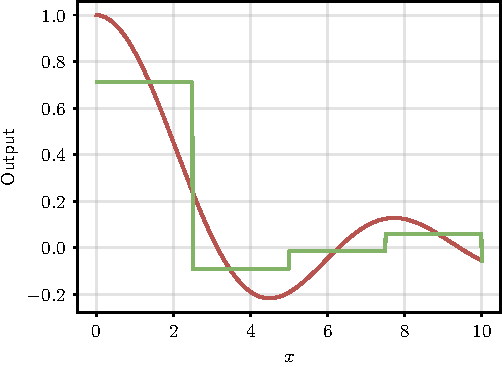
\includegraphics[width=0.95\textwidth]{images/sin_approximation_5.pdf}
    \caption{5 bins}
    \end{subfigure}
    \hfill
    \begin{subfigure}[b]{0.32\textwidth}
    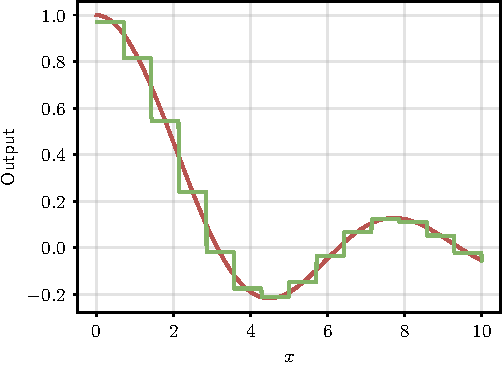
\includegraphics[width=0.95\textwidth]{images/sin_approximation_15.pdf}
    \caption{15 bins}
    \end{subfigure}
    \hfill
    \begin{subfigure}[b]{0.32\textwidth}
    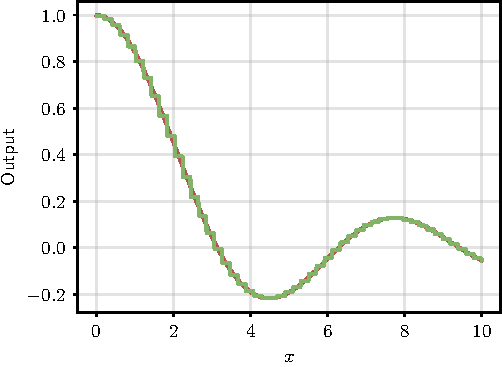
\includegraphics[width=0.95\textwidth]{images/sin_approximation_50.pdf}
    \caption{50 bins}
    \end{subfigure}
    \hfill
    \caption{Approximating $g(x) = \frac{\sin(x)}{x}$ in $[0,10]$ with (a) $m=5$, (b) $m=15$, and (c) $m=50$ bins. The original function is in red, the approximation \eqref{eq:proof_3} in green. The average squared error in the three cases decreases exponentially (approximately $0.02$, $0.002$, and $0.00016$).}
    \label{fig:sin_approximation}
\end{figure}

Similar reasonings can be applied to multi-dimensional inputs and different activation functions.\footnote{\url{http://neuralnetworksanddeeplearning.com/chap4.html}}